\section{Control system design}

\subsection{Problem a}

SPØR STUDASS HVORDAN man skal ta hensyn til $\psi$ i deloppgave b), c), og d). SVAR: Det er allerede tatt hensyn til ettersom psi holder seg innen 35 grader

FÅ INN FIGURER AV simulink modellene etter du finner ut hvordan dette gjøres mest hensiktsmessig.

The PD transfer function is of the form
\begin{align*}
    H_{pd}(s) &= K_{pd}(1+T_d s)/(1+T_f s) \\
              &= K_{pd}(1+T s)/(1+\alpha T s)
\end{align*}

Where $T_d = T$ in order to cancel the systems pole factor $(Ts + 1)$, and $T_f = \alpha T_d = \alpha T$. We set $K_{pd} = 0.8, \alpha = 0.1$. \Cref{fig:3a-bode_and_phasemargin} contains the bode plot of the system $H(s) = H_{ship}(s)H_{pd}(s)$, with the phase margin Pm at 48.3 degrees, and crossover angular frequency at 0.104 rad/s. ("DESCRIBE IN WORDS what can be seen in the plot"?)

Phase margin was found through the $margin(sys)$ MATLAB function, by using trial and error in placing $K_{pd}$ and $\alpha$. The $margin$ function calculates the phase margin by solving for the difference between the system phase and -180 degrees at the angular frequency where the systems amplitude is 1. (VURDER Å SKRIV OM. OGSÅ finn ut om dette er for nøye forklaring eller ikke)

\begin{figure}[ht]
    \centering
    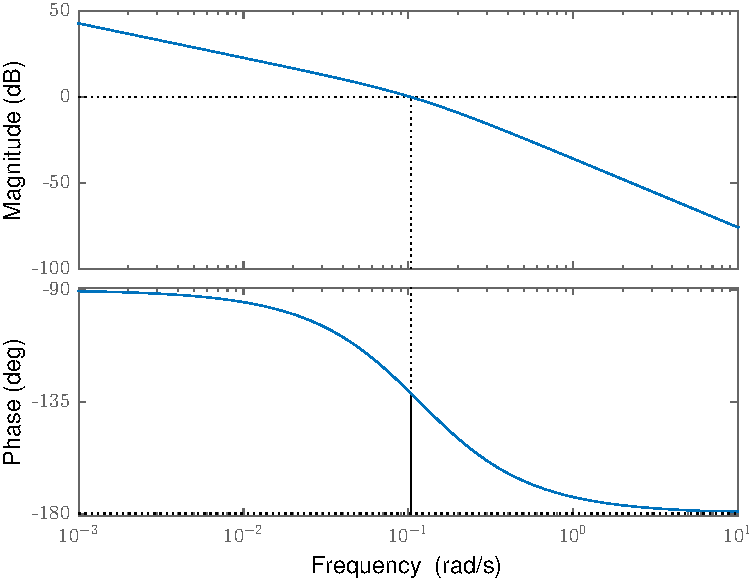
\includegraphics[width=0.5\textwidth]{images/3a-bode_and_phasemargin}
    \caption{Bode - and phase margin plot}
    \label{fig:3a-bode_and_phasemargin}
\end{figure}

\subsection{Problem b}
As shown in \cref{fig:3b-psi_and_rudder}, the autopilot functions with only measurement noise.

\begin{figure}[ht]
    \centering
    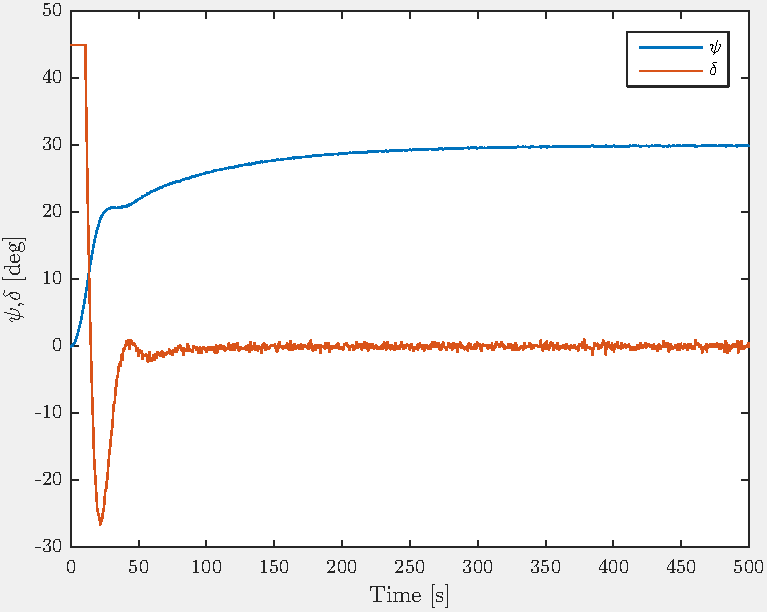
\includegraphics[width=0.5\textwidth]{images/3b-psi_and_rudder}
    \caption{Compass angle, $\psi$, and rudder angle, $\delta$, along the y-axis, plotted against time in the x-axis. With measurement noise}
    \label{fig:3b-psi_and_rudder}
\end{figure}

\subsection{Problem c}
As shown in \cref{fig:3b-psi_and_rudder_w_current}, the autopilot functions somewhat but has a stationary deviation as expected.

\begin{figure}[ht]
    \centering
    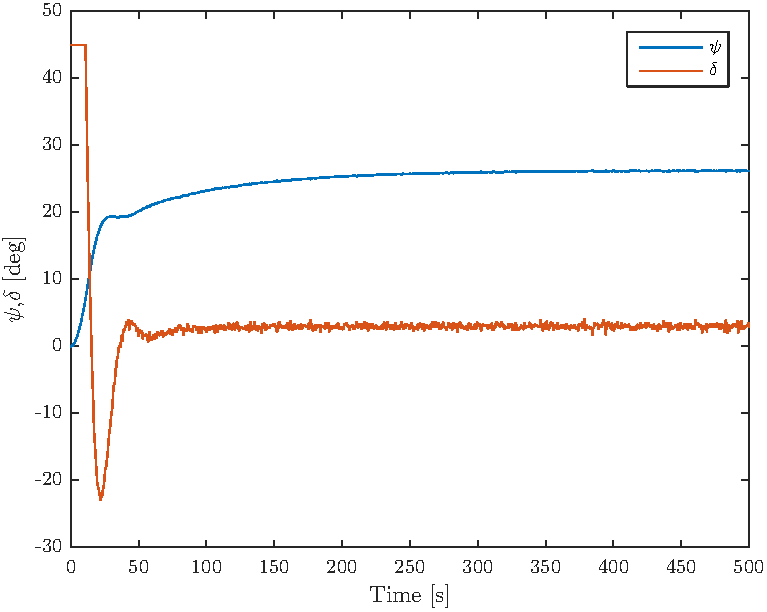
\includegraphics[width=0.5\textwidth]{images/3c-psi_and_rudder_w_current}
    \caption{Compass angle, $\psi$, and rudder angle, $\delta$, along the y-axis, plotted against time in the x-axis. With current disturbance and measurement noise}
    \label{fig:3b-psi_and_rudder_w_current}
\end{figure}

\subsection{Problem d}
As shown in \cref{fig:3b-psi_and_rudder_w_waves}, the autopilot functions somewhat but with unacceptable high frequent noise that would strain the motors of the ship. \todo{Snakk om hvordan kalman filteret kommer til å løse dette senere. Selv om det er åpenbart for oss er det ikke nødvendigvis åpenbart for retter om vi forstår det}

\begin{figure}[ht]
    \centering
    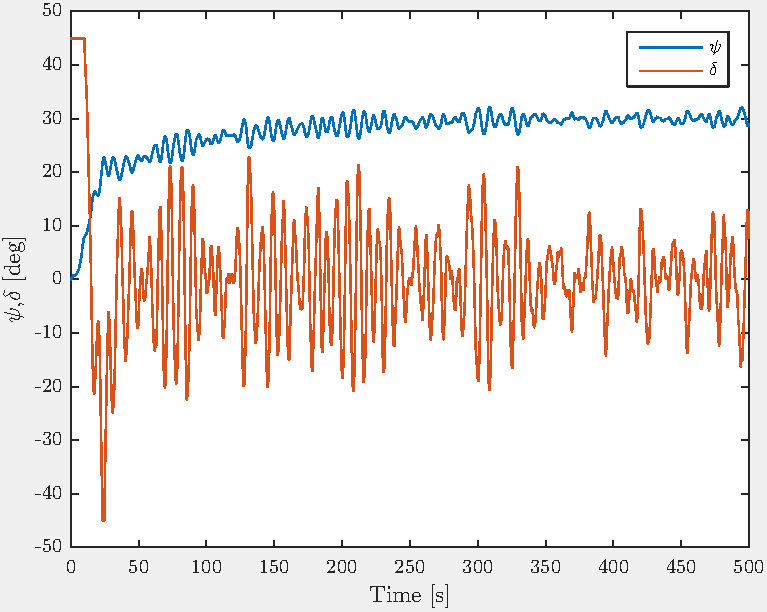
\includegraphics[width=0.5\textwidth]{images/3d-psi_and_rudder_w_waves}
    \caption{Compass angle, $\psi$, and rudder angle, $\delta$, along the y-axis, plotted against time in the x-axis. With wave disturbance and measurement noise}
    \label{fig:3b-psi_and_rudder_w_waves}
\end{figure}